\begin{frame}
  \titlepage
  \begin{figure}[ht]
      \begin{center}
          
\includegraphics[height=1in]{images/logo-taller.png}
      \end{center}
  \end{figure}
\end{frame}

\begin{frame}{Motivación 1/2}

    \begin{figure}[ht]
        \begin{center}
            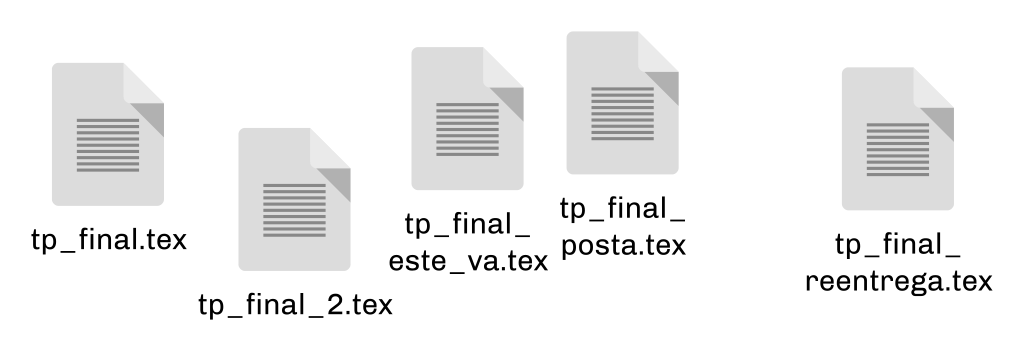
\includegraphics[height=1.5in]{images/caos.png}
        \end{center}
    \end{figure}

    \pause
    \begin{figure}[ht]
        \begin{center}
            
\includegraphics[height=1.5in]{images/horror.png}
        \end{center}
    \end{figure}

\end{frame}

\begin{frame}{Motivación 2/2}

    \begin{block}{Trabajando de a grupo}
        \begin{itemize}
            \item Enviar cambios por mail, o
            \pause
            \item Sincronizar cambios por Dropbox, o
            \pause
            \item Sincronizar cambios por Google Docs.
        \end{itemize}
    \end{block}

    \pause
    \begin{figure}[h]
        \begin{center}
            
\includegraphics[height=1.5in]{images/horror.png}
        \end{center}
    \end{figure}

\end{frame}

\begin{frame}{¿Qué es un Sistema de Control de Versiones?}

	\begin{block}{}
		Los Sistemas de Control de Versiones son una categoría de programas que permiten a un equipo manejar los cambios en el código fuente de un proyecto a lo largo del tiempo.

		Dichos programas llevan un seguimiento de las modificaciones que hacemos al código, y en caso de que nos equivoquemos en algo es posible volver a tras y comparar el código actual con otras versiones anteriores para ayudar a arreglar el error.

		También, permiten que varias personas distintas del equipo modifiquen el código a la vez y compartan los cambios, tratando que prevenir posibles conflictos, y en caso de que los hubiera ayudando a identificarlos y resolverlos.

	\end{block}

    \pause
    \begin{resumen}{Es decir..}
        \begin{itemize}
            \item Permiten arreglar \textit{accidentes} y volver a versiones anteriores del código.
            \item Permiten compartir código con otras personas.
        \end{itemize}
	\end{resumen}

\end{frame}

\begin{frame}{¿Qué es Git?}

	\begin{block}{}
		Git es un Sistema de Control de Versiones \textbf{distribuido y de código abierto}.
        Además fue diseñado con enfasis en la \textbf{performance} (para manejar proyectos muy grandes), \textbf{seguridad} y \textbf{flexibilidad}.
        Provee un amplio conjunto de comandos que permiten realizar operaciones de alto y bajo nivel.
	\end{block}

    \begin{figure}[ht]
        \begin{center}
            
\includegraphics[height=1.5in]{images/logo-git.png}
        \end{center}
    \end{figure}
\end{frame}

\begin{frame}[fragile]{Configuraciones iniciales}

	\begin{block}{Clave ssh}
		Para poder trabajar comodamente con repositorios Git que estén en internet (GitHub, Bitbucket, GitLab, etc) podemos configurar una clave ssh que nos identifique con el servidor que estemos usando.

        Por ejemplo, en GitLab:

        \url{http://doc.gitlab.com/ce/gitlab-basics/create-your-ssh-keys.html}
	\end{block}

    \begin{block}{Tu identidad}
        Es importante establecer nuestro nombre y email ya que estos van a ir asociados con los cambios que hagamos:

        \vspace{0.5em}

        \texttt{git config --global user.name "John Doe"}

        \texttt{git config --global user.email johndoe@example.com}
    \end{block}


\end{frame}

\begin{frame}[t]{Obteniendo un repositorio Git}

    \begin{comando}
        git clone
    \end{comando}

    \pause
	\begin{block}{}
        Para obtener una copia local de un repositorio existente en algún servidor,
        utilizamos el comando \texttt{git clone [URL]} (sin los corchetes)
    \end{block}

    \pause
    \vspace{1em}
    \begin{ejercicio}{Ejercicio}
        \textit{Clonar} el repositorio que tiene URL: \textbf{git@gitlab.com:talleres-comcom/taller-git.git}

        \vspace{0.5em}
        Es un repositorio que tiene los fuentes\ \LaTeX\ de estas diapositivas !
    \end{ejercicio}
\end{frame}

\begin{frame}[t]{Preparando cambios}
    \begin{comando}
        git add
    \end{comando}

    \pause
    \begin{block}{}
        Una vez que tenemos cambios hechos, tenemos que marcalos como \textit{preparados} (o listos) antes de confirmarlos.
        \begin{enumerate}
            \item Creamos/Modificamos el archivo en cuestión.
            \item Ejecutamos \texttt{git add [nombre del archivo]}
        \end{enumerate}
    \end{block}

    \pause
    \vspace{1em}
    \begin{ejercicio}{Ejercicio}
        Adentro del repositorio que \textit{clonaron} recién, crear un archivo y
        marcarlo como \textit{preparado} usando el comando \texttt{git add}.
    \end{ejercicio}
\end{frame}

\begin{frame}[t]{Confirmando cambios}
    \begin{comando}
        git commit
    \end{comando}

    \pause
    \begin{block}{}
        Una vez que tenemos \textit{preparados} ciertos cambios, podemos confirmarlos
        ejecutando \texttt{git commit -m [mensaje]}.

        \vspace{0.5em}

        Dónde [mensaje] índica al que lea eso cuales fueron los cambios que acabamos de confirmar.
    \end{block}

    \pause
    \vspace{1em}
    \begin{ejercicio}{Ejercicio}
        Confirmar los cambios que \textit{prepararon} en la diapo anterior.
    \end{ejercicio}
\end{frame}

\begin{frame}[t]{No seas vago con los mensajes!}

    \begin{figure}[ht]
        \begin{center}
            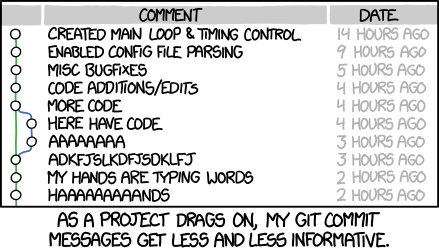
\includegraphics[height=2in]{images/xkcd-git-commit.png}
        \end{center}
        \caption{Fuente: \url{https://xkcd.com/1296/}}
    \end{figure}

\end{frame}

\begin{frame}[fragile, t]{¿Está preparado, confirmado o ninguna de las dos?}
    \begin{comando}
        git status
    \end{comando}

    \begin{block}{No es lo mismo!}
        Las modificaciones que hacemos pueden estar en \textbf{3 estados} distintos:
        \begin{itemize}
            \pause
            \only<-2>{\item \textbf{Modificado (modified)}: las modificaciones todavía no están \textit{preparadas o listas}.}
            \only<3-3>{\item \textbf{Preparado (staged)}: las modificaciones están marcadas como \textit{preparadas o listas} e
                irán en la proxima \textit{confirmación de cambios}.}
            \only<4-4>{\item \textbf{Confirmado (committed)}: las modifiaciones están guardadas con un \textit{mensaje} que explica los cambios realizados.}
        \end{itemize}
    \end{block}

    \only<2> {
        \begin{block}{Output de ejemplo}
            \gitstatusmodified
        \end{block}
    }
    \only<3> {
        \begin{block}{Output de ejemplo}
            \gitstatusready
        \end{block}
    }
    \only<4> {
        \begin{block}{Output de ejemplo}
            \gitstatusclean
        \end{block}
    }
\end{frame}

\begin{frame}{Colaborando con otras personas}

    Los repositorios remotos son \textit{copias} de tu proyecto a las cuales accedemos a través
    de Internet. Puede haber varios, cada uno de los cuales
    puede ser de sólo lectura, o de lectura/escritura, según los permisos que tengamos.

    \begin{figure}[ht]
        \begin{center}
            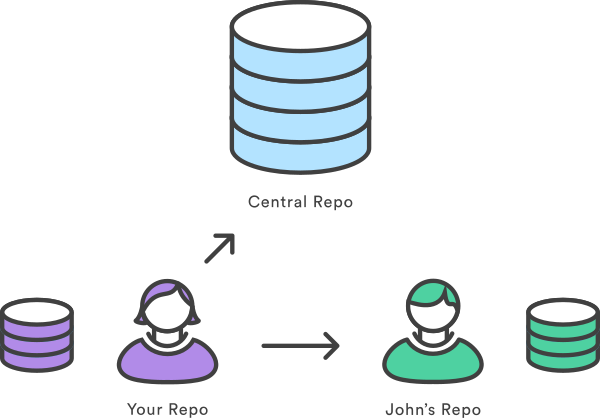
\includegraphics[height=1in]{images/repo-remoto.png}
        \end{center}
    \end{figure}

    Colaborar con otros implica gestionar estos repositorios remotos, y mandar (\textbf{push}) y recibir (\textbf{pull})
    datos de ellos cuando necesites compartir cosas.

\end{frame}

\begin{frame}[t]{Enviando cambios}
    \begin{comando}
        git push
    \end{comando}

    \pause
    \begin{block}{}
        Para enviar los cambios \textbf{desde nuestro repositorio local a algún
        repositorio remoto}, ejecutamos: \texttt{git push [remoto] [branch]}

        \vspace{0.5em}

        Por ahora, hasta la siguiente clase, vamos a usarlo como:\\ \texttt{git push origin master}
    \end{block}
\end{frame}

\begin{frame}[t]{Trayendo cambios}
    \begin{comando}
        git pull
    \end{comando}

    \pause
    \begin{block}{}
        Para traer cambios \textbf{desde un repositorio remoto a nuestro repositorio local},
        ejecutamos: \texttt{git pull [remoto] [branch]}

        \vspace{0.5em}

        Igual que antes, hasta la siguiente clase, vamos a usarlo como:\\ \texttt{git pull origin master}
    \end{block}
\end{frame}

\begin{frame}[t]{Y qué pasa sí.. BOOM}

    \begin{block}{A veces hay conflictos}
        \begin{itemize}
            \item Supongamos que dos personas (👨 y 👩) están trabajando en un mismo proyecto.
                Es decir, ambos tienen una \textit{copia} en su máquina.
            \pause
            \item Ahora imaginemos, por ejemplo, que 👨 modifica el archivo \texttt{README} en la linea 23
                y confirma los cambios.
            \pause
            \item Sin saberlo, 👩 también modifica el archivo \texttt{README} en la linea 23, pero pone algo distinto y confirma dichos cambios.
            \pause
            \item ¿Qué va a pasar cuando quieran compartir lo que hicieron?\\ \only<6->{Va a haber un conflicto,
                dos personas dicen algo distinto para una misma lniea.}
            \pause
            \item ¿Que va a hacer Git?\\ \only<7->{Se va a quejar. A alguno de los dos le va a tocar incorpar \textbf{a mano} los cambios del otro.}
        \end{itemize}
    \end{block}

\end{frame}

\begin{frame}[t]{Creando un repositorio vacio}
    \begin{comando}
        git init
    \end{comando}

    \pause
    \begin{block}{}
        Crea un repositorio local vacio. Un lienzo en blanco por así decirlo.
        \begin{enumerate}
            \item Nos paramos en el directorio que queremos convertir en un repositorio.
            \item Ejecutamos \texttt{git init}
        \end{enumerate}
        Esto crea un subdirectorio \textit{.git} que tiene todos los archivos necesarios de Git.
    \end{block}
\end{frame}

\begin{frame}[t]{Añadiendo un repositorio remoto}
    \begin{comando}
        git remote
    \end{comando}

    \vspace{0.5em}
    \pause
    \begin{block}{Ver los repositorios remotos asociados}
        Ejecutamos \texttt{git remote -v}
    \end{block}

    \pause
    \begin{block}{Agregar un repositorio remoto}
        Ejecutamos \texttt{git remote add [nombre que querramos] [URL]}
    \end{block}
\end{frame}

\begin{frame}[t]{A practicar!}
    Ejercicio de a 2 máquinas (preferiblemente 2 personas): 👾 y 👽

    \begin{enumerate}
        \pause
        \item 👾 y 👽: crear un repositorio local vacio.
        \pause
        \item 👾: crear un repositorio nuevo en \href{https://www.gitlab.com}{GitLab}
        \pause
        \item 👾 y 👽: asociar el repositorio remoto recién creado.
        \pause
        \item 👾 y 👽: crear un archivo \textit{README} con contenidos distintos en la primera linea.
        \pause
        \item 👾: pushear los cambios al repositorio remoto.
        \pause
        \item 👽: intentar pushear los cambios al repositorio remoto. ¿Qué pasó?
        \pause
        \item 👽: bajarse los cambios del repositorio remoto. ¿Anduvo?
        \pause
        \item 👽: resolver los conflictos que haya.
        \pause
        \item 👽: añadir y confirmar el archivo que tenía conflicto.
        \pause
        \item 👽: pushear estos nuevos cambios.
        \pause
        \item 👾: bajarse los nuevos cambios.
    \end{enumerate}
\end{frame}
